\documentclass[html]{report}    % Specifies the document style.
\usepackage{graphicx}
                           % The preamble begins here. 
\title{Multi-Agent Systems Project}  % Declares the document's title. 
\author{Chatzichristodoulou Panagiotis , Tumanov Kirill}    % Declares the author's nam
\date{November 29,2013}   % Deleting this command produces today's date.


\begin{document}           % End of preamble and beginning of text.

\maketitle                 % Produces the title.

In this paper, we will discuss our analysis and implementation of a negotiating agent, as part of our Multi-Agent systems course.
\section{Acceptance Strategy}  % Produces section heading.  Lower-level 
                         % sections are begun with similar 
                         % \subsection and \subsubsection commands.
\subsection{Basic Definitions}                        
The acceptance strategy of the agent was based on the ABiNeS agent's ~\cite{abines} acceptance strategy.
The Acceptance strategy module introduces the acceptance threshold $\ell$ . The value of $\ell$ corresponds to the agents concession degree and is modified during the negotiation.  This change is based on the previous results of the negotiation as well as to the negotiation environment.


The agent is build as a self-interested agent and will be more concessive as the deadline approaches.
The acceptance threshold should always be higher than the utility the agent can obtain on deadline. Therefore, the threshold should never be lower than the  \( Utility_{max} * discount_{time-1}  \) , where \( Utility_{max} \)  is the maximum utility the agent can receive without taking into account the discount factor. In contrast to this, if the agent takes too long to reach an agreement, it may receive very low utility due to the discount factor even if the agreed outcome proposes a high utility . For this, we introduce $\lambda$, a factor to balance of between exploring and exploiting the negotiating partner.
More formally, when time is smaller than $\lambda$, it should be modified to gradually converge to \( Utility_{max} * discount_{time-1}  \). So the $\ell$ is defined as follows:


\[
  \ell = \left\{\def\arraystretch{1.2}% 
  \begin{array}{@{}c@{\quad}l@{}}
    u^m -(u^m-	u^md^t)(t/\lambda)^a  & \mbox{if } t \geq \lambda \\
   	u^m d^t & \mbox{if } t < \lambda
  \end{array}\right.
\]

\[
  \lambda = \left\{\def\arraystretch{1.2}%
  \begin{array}{@{}c@{\quad}l@{}}
    \lambda = \lambda_0 + (1-\lambda_0)^b &  \mbox{if } t==0\\
    \lambda = \lambda + w(1-\lambda_0)\sigma^t & \mbox{if } 0<t\leq1\\
  \end{array}\right.
\]

So as time increases, $\ell$ will decrease slowly, and as time reaches $\lambda$ , $\ell$ will be set to\( Utility^{max} * discount^{time}  \).
\\*Graphically, this can be presented as:


	\begin{figure}[h!]
	  \caption{Change of $\ell$ over time .}
	  \centering
	    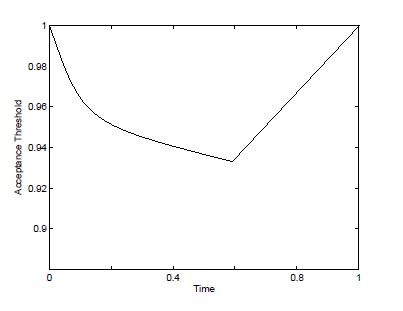
\includegraphics[width=0.5\textwidth]{ell}
	\end{figure}

\section{Bids offering Strategy}

Agent's bid offering strategy was implemented as time-dependent. The NegoAgent\_TDOffering.class requires two user parameters: $P_{min}$ and $P_{max}$ which specify the lower and upper bounds for the bids agent is to propose. In the current version of the agent these values were kept equal to $0$ and $0.99$ respectfully. No experimentation was done on changing these values, it may be the case that some alterations in specific negotiation domains are beneficial, however this topic is left for an additional research.

Offering strategy introduces two methods used in the agent: \textit{isNash()} and \textit{countUniqueBids()}. First one is a simple implementation of the two-factor (due to the number of negotiating parties) maximization algorithm. An idea behind it is in finding a Nash equilibrium point, there none of the parties can obtain a higher utility at no cost to any other party. This particular implementation does not claim to be optimal, but it produced sufficiently good results for the agent at this stage of development. The pseudo-code of the  \textit{isNash()} method is given as follows:

\begin{verbatim}
	public boolean isNash()
	{
		BidHistory bH = negotiationSession.getOpponentBidHistory();
		
		if (bH.getLastBidDetails().getBid() != null)
		{
			double temp = bH.getLastBidDetails().getMyUndiscountedUtil() + opponentModel.getBidEvaluation(bH.getLastBidDetails().getBid());
			
			if (temp < nashsum && opponentModel.getBidEvaluation(bH.getLastBidDetails().getBid()) < bH.getBestBidDetails().getMyUndiscountedUtil())
				return true;
			else
				nashsum = temp;
		}
		
		return false;
	}
\end{verbatim}

\subsection{Acceptance Model}

Now that we have defined the environment, the acceptance condition is a function of the history of the previous negotiations, the current acceptance threshold, and the outcome of the negotiation at time t.
\\*The agent will accept a proposal $\pi$ if he receives utility bigger than his current threshold, or his next-bid to propose utility.


\section{Opponent Model}  

The opponent model is based on the Hard Headed Opponent model of the genius-BOA framework.
\\*Besides from the basic model, there are two extra components in the model.~\cite{anac2013}
\subsection{Simple Frequency}
The Simple frequency model only updates weights when the bid change often.
That means that the weights of the model are only changed when the opponents bids pass a certain numerical threshold.
\subsection{Distance of the opponent}
The opponent model also calculates a threshold that is used in the Acceptance strategy and is based on the distance of the opponent.
\\{\bf The basic algorithm of the distance of the opponent is: }

DOUS = u$^m - firstOppBid \newline
calculate\ mean\ and\ variance\ foreach\ past\ bid\ where:\newline
firstOppBid< bidUtil<u^m \newline
use\ the\ (mean+dous)/2\ as\ a\ threshold\ value\ if\ time<.5 \newline
if(time<.5)\space return \ threshold \ else \ return \ 0$

The visualization of the DOUS distance would be:
\begin{figure}[h!]
  \caption{The distance between the initial utilities of the agents.}
  \centering
    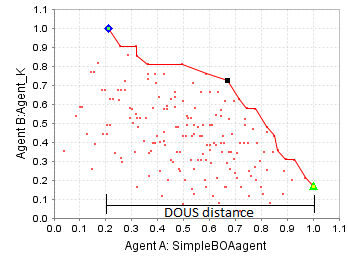
\includegraphics[width=0.5\textwidth]{dous}
\end{figure}


The DOUS value is versatile, as it is not domain dependent.
As it is presented here, it can be implemented only on negotiations of two agents, but it can be expanded to multiple agent negotiations.
The thershold is outputed is weak threshold.
That is, if the value is smaller than the threshold, the bid is rejected.If the value is higher, we compare it with the normal threshold computed in the Acceptance Strategy.
This threshold ensures that the agents will reject points that are far from the nash equilibrium.
After some time in the negotiation, the threshold is set to zero, because the agent needs to be more concessive as the negotiation approaches the deadline. 

\section{Binding the modules together}

In order to bind all the modules together, we created a class that extended the BOA agent and passed each all the modules, as parts of the agent with their parameters set. We then only have to override the agent setup method of the class.  The code of the overriden class is:


\begin{verbatim}
	NegoAgent extends BOAagent {
    
    @Override
    public void agentSetup(){
        OpponentModel om = new OpponentsModel(negotiationSession);
        OMStrategy oms = new BidStrategy(negotiationSession , om);
        OfferingStrategy offering = new NegoAgent_TDOffering(nego
        tiationSession, om, oms, 1D, 0D, .99D, 0D);
        AcceptanceStrategy ac =  new AStrategy(negotiationSession,
         offering, .2D , 15D);
        setDecoupledComponents (ac , offering , om , oms );
    }
    @Override
    public String getName () {
        return " SimpleBOAagent ";
    }
}
\end{verbatim}
Now, we can update the negosimulator jar to include the class, or just insert it from the gui.







\begin{thebibliography}{5}

\bibitem{abines} Jianye Haoand Ho-fung Leung,ABiNeS:

\bibitem{anac2013} Jianye Haoand Ho-fung Leung,ABiNeS: An Adaptive Bilateral Negotiating Strategy over Multiple Items
\end{thebibliography}

\end{document}             % End of document. 